\section{Rendering Markdown Text}
\label{sec:markup}

Once the chapters are known, each of them has to become a list of content blocks, most of which are
Text blocks carrying HTML.
This section covers the constructs that can be expressed as markup inside a Text block: text,
headings, lists, emphasis, block quotes, and code.
Images, tables, and the constructs that enclose them require separate content blocks.

Every decision in this section depends on \autoref{tab:allowed}, which lists what survives the
sanitizer in the two libraries the converter writes text into.
The upper half lists, per tag, whether a Text block and a Table block keep it and whether it may
carry a \code{style} attribute; the lower half lists which declarations inside that attribute
are kept.
The table was derived from the sanitizer implementation and the \code{semantics.json} of both
libraries\footnote{\raggedright Tags: \code{validateText} in
\code{h5p.classes.php}, lines 4303--4327, starting from the library's \code{tags} array and
always adding \code{div}, \code{span}, \code{p}, and \code{br}; styleable tags:
\code{\$allowed\_styleable\_tags}, lines 4201--4214; declarations: \code{\$stylePatterns}, lines
4330--4376, unlocked per library by its \code{font} block and by \code{table} being among its
tags.}~\cite{H5P:PhpLibrary}.
Two of its properties shape the rest of the conversion.
First, the rules differ per library: \code{table} is allowed in a Table block but not in a Text
block; \code{border} and \code{padding} exist only for libraries that permit \code{table}.
Second, the rules cannot be changed.
A library's \code{semantics.json} is part of the package, but the platform keeps the copy it already
has installed, so a modified one would be ignored.

\begin{table}[H]
	\centering
	\small
	\begin{tabular}{@{}>{\raggedright\arraybackslash}p{0.45\columnwidth}cc>{\raggedright\arraybackslash}p{0.24\columnwidth}@{}}
		\toprule
		\textbf{Tag} & \textbf{AdvancedText} & \textbf{Table} & \textbf{Styleable} \\
		\midrule
		\code{div}, \code{span}, \code{p} & \tyes & \tyes & \tyes \\
		\code{br}, \code{strong}, \code{em}, \code{del}, \code{s}, \code{a}, \code{code} & \tyes & \tyes & \tno \\
		\code{h2}, \code{h3}, \code{li} & \tyes & \tno & \tyes \\
		\code{ul}, \code{ol}, \code{hr}, \code{pre} & \tyes & \tno & \tno \\
		\code{table}, \code{td}, \code{th}, \code{col}, \code{figure} & \tno & \tyes & \tyes \\
		\code{tr}, \code{thead}, \code{tbody}, \code{tfoot}, \code{colgroup}, \code{figcaption} & \tno & \tyes & \tno \\
		\midrule\midrule
		\textbf{Style Declaration} & \textbf{AdvancedText} & \textbf{Table} & \textbf{Unlocked by} \\
		\midrule
		\code{text-align} & \tyes & \tyes & every text \\
		\code{color} & \tyes & \tyes & \code{font} semantics \\
		\code{font-size} & \tyes & \tno & \code{font} semantics \\
		\code{background-color} & \tyes & \tyes & \code{font} semantics; table group \\
		\code{border}, \code{border-style}, \code{border-width}, \code{border-color}, \code{border-collapse}, \code{padding}, \code{vertical-align}, \code{width}, \code{height}, \code{float} & \tno & \tyes & table group \\
		\bottomrule
	\end{tabular}
	\caption[What survives H5P's sanitizer in a Text block and a Table block]{\label{tab:allowed}What survives H5P's sanitizer in the two libraries the converter
		writes text into.
		Styleable says whether a \code{style} attribute is kept on the tag at
		all; a declaration inside it then has to pass the lower half, where table group is the
		set unlocked for any library whose semantics permit \code{table}.
		Anything not listed is
		dropped silently.
		Derived from the sanitizer implementation and the libraries'
		\code{semantics.json}, not from documentation.}
\end{table}

\subsection{Document Traversal}
\label{sec:mk_visitor}

commonmark-java includes an HTML renderer, but the converter does not use it.
The sanitizer removes a tag it does not permit and keeps its text, so a \code{blockquote} produced by
the renderer would silently turn into an ordinary paragraph.
Such a loss is only noticed by comparing the source with the book.
Post-processing the renderer's output would mean parsing the HTML again and rewriting every tag the
platform does not accept.
Moreover, the mapping is not one tag to another: a block quote becomes a \code{div} with a label and
a background.
The converter therefore renders the node tree itself and only emits markup that survives, so
every deviation from the Markdown is intentional.

\begin{figure}[H]
	\centering
	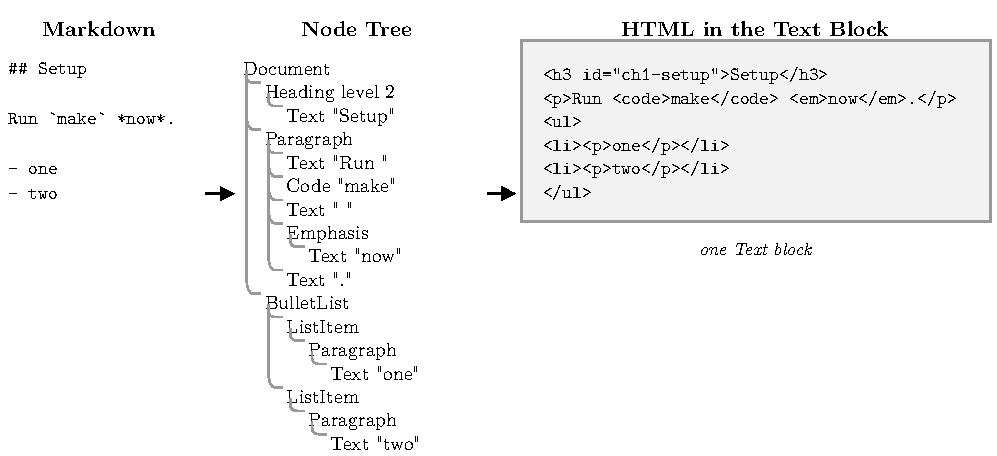
\includegraphics[width=\columnwidth]{figures/render-tree}
	\caption[From Markdown to the node tree to HTML]{\label{fig:render_tree}A Markdown fragment, the node tree the parser produces, and the
		HTML the visitor emits.
		The heading, emphasis, and list
		each map onto a permitted tag; the whole fragment lands in a single Text block.}
\end{figure}

The parser produces a tree in which a document holds block nodes, blocks hold inline nodes, and
every node type is a class.
To traverse this tree, the converter uses a visitor with one method per node type.
Nearly every method opens a tag, renders the children, and closes the tag.
For example, \autoref{lst:emphasis_visitor} shows how the emphasis visitor wraps its children in
\code{em}.

\begin{lstlisting}[language=Kotlin,
caption={[The emphasis visitor]The emphasis visitor.},label={lst:emphasis_visitor}]
override fun visit(emphasis: Emphasis) {
    html.pushTag("em")
    visitChildren(emphasis)
    html.popTag()
}
\end{lstlisting}

\autoref{fig:render_tree} shows a short fragment, its tree, and the resulting HTML.
A heading becomes an \code{h3} with an anchor, an emphasis
node becomes \code{em}, and a list becomes \code{ul} with one \code{li} per
item.
All of it is collected in one buffer that is finally written into one Text block.

The visitor keeps two pieces of state.
The first is a \emph{tag stack}: every opened tag is pushed and every closed tag popped, so the
converter always knows which tags are open.
This is needed when something interrupts the text: the open
tags are closed, the interruption is emitted, and the same tags are opened again afterward.
A tag that contains nothing or only whitespace is dropped when it is popped, so that no empty
\code{<p></p>} or empty list item remains after an interruption.
The second is a \emph{text buffer}: it collects the generated HTML until something forces a break.
Flushing writes its contents into a Text block and clears the buffer for the next stretch of text.
A chapter that contains only text is therefore flushed once at its end and becomes a single block.

\subsection{Mapping Constructs to Markup}
\label{sec:mk_easy}

For each construct, the converter has to decide which tag to emit.
For many constructs this is the obvious tag, while the rest need a substitute.

\paragraph{Directly Supported Constructs.}
Paragraphs, emphasis, strong emphasis, inline code, links, ordered and unordered lists, thematic
breaks, and strikethrough have their usual tag in the upper half of \autoref{tab:allowed}.
The converter emits \code{p}, \code{em}, \code{strong}, \code{code}, \code{a}, \code{ul}, \code{ol},
\code{li}, \code{hr}, and \code{del}.
Links also need attributes that identify their destination.

\paragraph{Block Quotes and Alerts.}
\code{blockquote} is permitted in no library.
The same holds for the alerts of GitHub Flavored Markdown, which are block quotes with a marker such
as \code{[!NOTE]} or \code{[!WARNING]}.
Among the permitted options, only a background color makes a passage look like a separate box, and
only a \code{div} can contain block content such as a list, a code block, or a nested quote.
A block quote therefore becomes a \code{div} with a light gray \code{background-color} and a
speech-bubble emoji as its label.
An alert gets the emoji and label of its type.
Since \code{border} and \code{padding} are not available outside the table libraries, nested boxes
cannot be told apart by their frame.
The shade therefore darkens by one step per nesting level, starting from \code{\#f2f2f2}, for up to
ten levels.

Two alternatives were rejected.
A \code{pre} element is in the tag list, but it is not styleable, so it cannot be shaded. It also may
not contain a list or a code block.
A one-cell Table block would have a real frame, since \code{border} and \code{padding} are available
there, but a table cell may not contain \code{ul}, \code{ol}, \code{h2}, or \code{pre}, so any
structured quote would be flattened.

\paragraph{Headings.}
A Text block permits only \code{h2} and \code{h3}.
Since \code{h1} is not available, every heading is shifted down one level and clamped:
\code{\#} becomes \code{h2}, and \code{\#\#} and every deeper level become
\code{h3}.
Emitting \code{h4} to \code{h6} is not an option, because the sanitizer would remove them and turn
the headings into body text.
Representing deep headings as bold paragraphs would keep the levels distinguishable, but they would no longer be
headings.
Retaining a heading tag matters in Interactive Book, because its sidebar lists every \code{h2} and \code{h3} of a
chapter as a navigation target.
A clamped \code{h3} is therefore still an entry in the table of contents, but the distinction among levels below two is lost.

\paragraph{Inserted Text.}
The \code{++inserted++} extension marks text as added, but neither \code{ins} nor \code{u} is
permitted.
Bold or italic would be indistinguishable from ordinary emphasis, so inserted text becomes a
\code{span} with a light green \code{background-color}.
Deleted text is not colored red, although diffs usually show it that way.
A Markdown viewer renders \code{\textasciitilde\textasciitilde{}text\textasciitilde\textasciitilde}
as a plain strikethrough, and the book should look like the Markdown preview.

\paragraph{Task Lists and Footnote Marks.}
Two constructs are replaced by characters.
A task list item, \code{- [x]} or \code{- [ ]}, becomes a checked or empty box character in front of
the item text, since \code{input} is not permitted.
The box would not have been interactive anyway, because the platform does not store its state.
Similarly, a footnote reference becomes \code{[1]} on the baseline, since \code{sup} is not permitted either.

\begin{figure}[H]
	\centering
	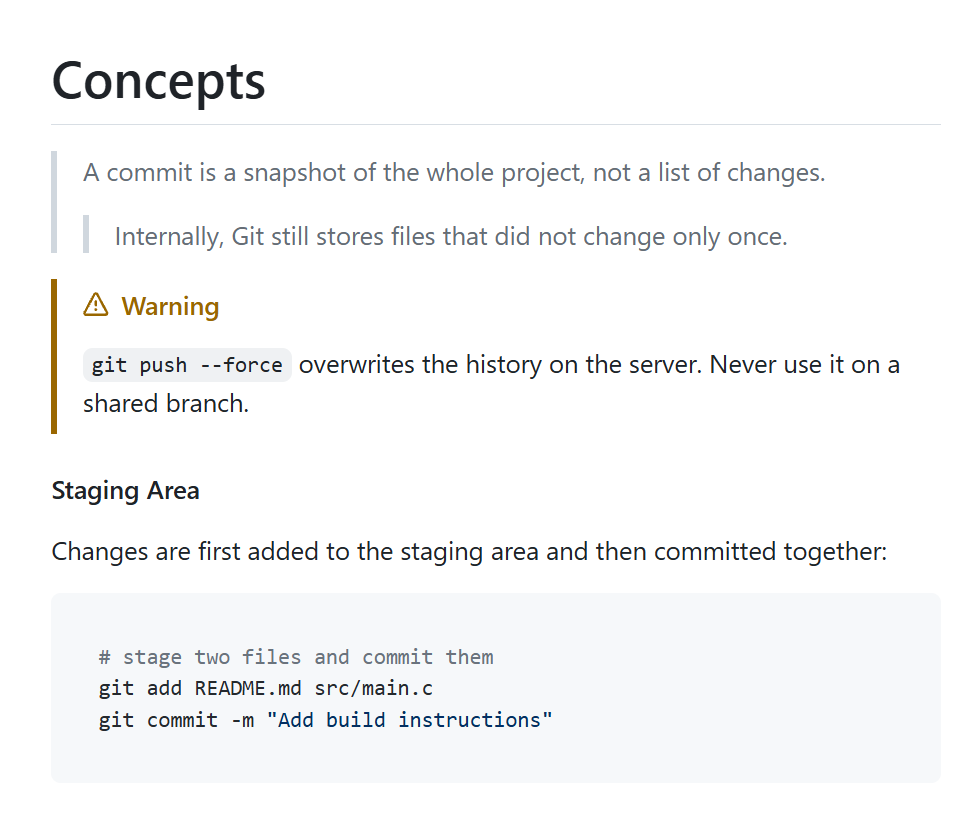
\includegraphics[height=0.45\columnwidth]{figures/screenshots/substitutes-preview}\hfill
	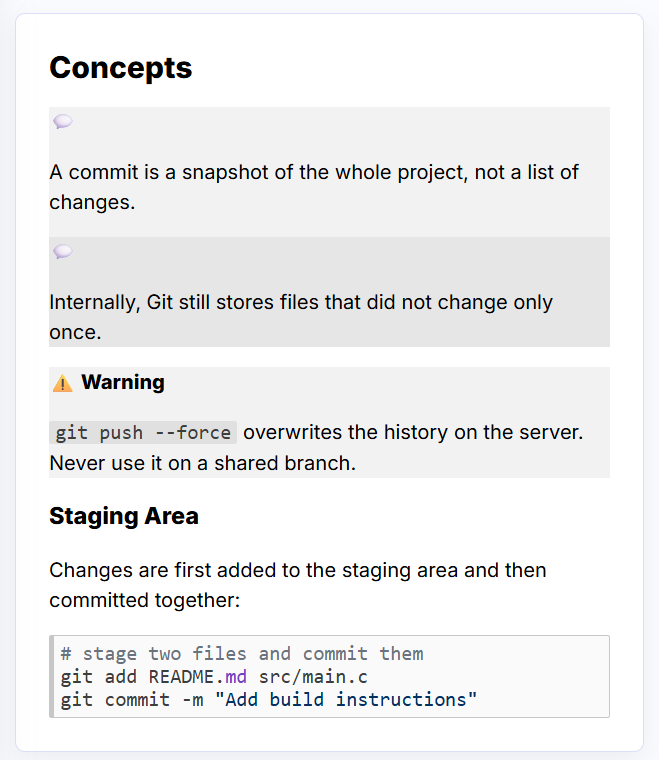
\includegraphics[height=0.45\columnwidth]{figures/screenshots/substitutes-moodle}
	\caption[Substitutes for unsupported tags next to a Markdown preview]{\label{fig:substitutes}The substitutes for unsupported tags next to the Markdown
		preview they stand in for.}
\end{figure}

\paragraph{Code Blocks.}
A fenced code block becomes \code{pre} and \code{code}, which are both permitted.
Without further styling, however, it is plain monospace text on the page background, since
\code{pre} is not styleable and no H5P stylesheet styles it.
The converter therefore wraps it in a \code{div} with a light background, as for block quotes.
The shade differs from the block quote grays, so that a code block inside a block quote remains
visible.
\autoref{fig:substitutes} shows the substitutes of this section next to the Markdown preview.

\subsection{Raw HTML}
\label{sec:mk_rawhtml}

Markdown permits raw HTML, both as a block and inline, and documentation written for the web uses
it for things Markdown lacks, such as a centered image or a collapsible section.
Mapping every HTML tag to something the platform accepts would mean guessing the author's intent,
and rejecting raw HTML would break documents that work everywhere else.
The converter therefore passes raw HTML through unchanged.
Moodle's sanitizer then removes the tags it does not allow.
Many of them are permitted anyway, such as \code{div}, \code{p}, \code{span}, \code{a}, and
\code{strong}.

The converter does emit warnings, however.
All raw HTML fragments are collected and checked at the end of the chapter
against the tag list of \autoref{tab:allowed} and for balanced tags.
The check covers the whole chapter, because a tag opened in one inline fragment and closed in
another is balanced.
Balance matters because Moodle's sanitizer is a regular-expression filter that does not repair the
markup\footnote{\raggedright \code{filter\_xss} in \code{h5p.classes.php}, lines 4912--5023, a port of
Drupal's filter of the same name.}~\cite{H5P:PhpLibrary}, so an unclosed tag remains open and can affect the rest of the
page.
The warning names the tags that will be removed and the tags that are not closed.
The converter does not repair either.
